\documentclass[11 pt,]{article}
\usepackage{lmodern}
\usepackage{amssymb,amsmath}
\usepackage{ifxetex,ifluatex}
\usepackage{fixltx2e} % provides \textsubscript
\ifnum 0\ifxetex 1\fi\ifluatex 1\fi=0 % if pdftex
  \usepackage[T1]{fontenc}
  \usepackage[utf8]{inputenc}
\else % if luatex or xelatex
  \ifxetex
    \usepackage{mathspec}
  \else
    \usepackage{fontspec}
  \fi
  \defaultfontfeatures{Ligatures=TeX,Scale=MatchLowercase}
    \setmainfont[]{Times}
\fi
% use upquote if available, for straight quotes in verbatim environments
\IfFileExists{upquote.sty}{\usepackage{upquote}}{}
% use microtype if available
\IfFileExists{microtype.sty}{%
\usepackage{microtype}
\UseMicrotypeSet[protrusion]{basicmath} % disable protrusion for tt fonts
}{}
\usepackage[margin=1in]{geometry}
\usepackage{hyperref}
\PassOptionsToPackage{usenames,dvipsnames}{color} % color is loaded by hyperref
\hypersetup{unicode=true,
            pdftitle={{[}Title{]}},
            pdfauthor={Karl Abuan; May Ho; Jonah Lin; Leilynaz Malekafzali; Tiffany Yang; Abdur Rahman M. A. Basher},
            colorlinks=true,
            linkcolor=Maroon,
            citecolor=Blue,
            urlcolor=blue,
            breaklinks=true}
\urlstyle{same}  % don't use monospace font for urls
\usepackage{color}
\usepackage{fancyvrb}
\newcommand{\VerbBar}{|}
\newcommand{\VERB}{\Verb[commandchars=\\\{\}]}
\DefineVerbatimEnvironment{Highlighting}{Verbatim}{commandchars=\\\{\}}
% Add ',fontsize=\small' for more characters per line
\usepackage{framed}
\definecolor{shadecolor}{RGB}{248,248,248}
\newenvironment{Shaded}{\begin{snugshade}}{\end{snugshade}}
\newcommand{\KeywordTok}[1]{\textcolor[rgb]{0.13,0.29,0.53}{\textbf{#1}}}
\newcommand{\DataTypeTok}[1]{\textcolor[rgb]{0.13,0.29,0.53}{#1}}
\newcommand{\DecValTok}[1]{\textcolor[rgb]{0.00,0.00,0.81}{#1}}
\newcommand{\BaseNTok}[1]{\textcolor[rgb]{0.00,0.00,0.81}{#1}}
\newcommand{\FloatTok}[1]{\textcolor[rgb]{0.00,0.00,0.81}{#1}}
\newcommand{\ConstantTok}[1]{\textcolor[rgb]{0.00,0.00,0.00}{#1}}
\newcommand{\CharTok}[1]{\textcolor[rgb]{0.31,0.60,0.02}{#1}}
\newcommand{\SpecialCharTok}[1]{\textcolor[rgb]{0.00,0.00,0.00}{#1}}
\newcommand{\StringTok}[1]{\textcolor[rgb]{0.31,0.60,0.02}{#1}}
\newcommand{\VerbatimStringTok}[1]{\textcolor[rgb]{0.31,0.60,0.02}{#1}}
\newcommand{\SpecialStringTok}[1]{\textcolor[rgb]{0.31,0.60,0.02}{#1}}
\newcommand{\ImportTok}[1]{#1}
\newcommand{\CommentTok}[1]{\textcolor[rgb]{0.56,0.35,0.01}{\textit{#1}}}
\newcommand{\DocumentationTok}[1]{\textcolor[rgb]{0.56,0.35,0.01}{\textbf{\textit{#1}}}}
\newcommand{\AnnotationTok}[1]{\textcolor[rgb]{0.56,0.35,0.01}{\textbf{\textit{#1}}}}
\newcommand{\CommentVarTok}[1]{\textcolor[rgb]{0.56,0.35,0.01}{\textbf{\textit{#1}}}}
\newcommand{\OtherTok}[1]{\textcolor[rgb]{0.56,0.35,0.01}{#1}}
\newcommand{\FunctionTok}[1]{\textcolor[rgb]{0.00,0.00,0.00}{#1}}
\newcommand{\VariableTok}[1]{\textcolor[rgb]{0.00,0.00,0.00}{#1}}
\newcommand{\ControlFlowTok}[1]{\textcolor[rgb]{0.13,0.29,0.53}{\textbf{#1}}}
\newcommand{\OperatorTok}[1]{\textcolor[rgb]{0.81,0.36,0.00}{\textbf{#1}}}
\newcommand{\BuiltInTok}[1]{#1}
\newcommand{\ExtensionTok}[1]{#1}
\newcommand{\PreprocessorTok}[1]{\textcolor[rgb]{0.56,0.35,0.01}{\textit{#1}}}
\newcommand{\AttributeTok}[1]{\textcolor[rgb]{0.77,0.63,0.00}{#1}}
\newcommand{\RegionMarkerTok}[1]{#1}
\newcommand{\InformationTok}[1]{\textcolor[rgb]{0.56,0.35,0.01}{\textbf{\textit{#1}}}}
\newcommand{\WarningTok}[1]{\textcolor[rgb]{0.56,0.35,0.01}{\textbf{\textit{#1}}}}
\newcommand{\AlertTok}[1]{\textcolor[rgb]{0.94,0.16,0.16}{#1}}
\newcommand{\ErrorTok}[1]{\textcolor[rgb]{0.64,0.00,0.00}{\textbf{#1}}}
\newcommand{\NormalTok}[1]{#1}
\usepackage{graphicx,grffile}
\makeatletter
\def\maxwidth{\ifdim\Gin@nat@width>\linewidth\linewidth\else\Gin@nat@width\fi}
\def\maxheight{\ifdim\Gin@nat@height>\textheight\textheight\else\Gin@nat@height\fi}
\makeatother
% Scale images if necessary, so that they will not overflow the page
% margins by default, and it is still possible to overwrite the defaults
% using explicit options in \includegraphics[width, height, ...]{}
\setkeys{Gin}{width=\maxwidth,height=\maxheight,keepaspectratio}
\IfFileExists{parskip.sty}{%
\usepackage{parskip}
}{% else
\setlength{\parindent}{0pt}
\setlength{\parskip}{6pt plus 2pt minus 1pt}
}
\setlength{\emergencystretch}{3em}  % prevent overfull lines
\providecommand{\tightlist}{%
  \setlength{\itemsep}{0pt}\setlength{\parskip}{0pt}}
\setcounter{secnumdepth}{5}
% Redefines (sub)paragraphs to behave more like sections
\ifx\paragraph\undefined\else
\let\oldparagraph\paragraph
\renewcommand{\paragraph}[1]{\oldparagraph{#1}\mbox{}}
\fi
\ifx\subparagraph\undefined\else
\let\oldsubparagraph\subparagraph
\renewcommand{\subparagraph}[1]{\oldsubparagraph{#1}\mbox{}}
\fi

%%% Use protect on footnotes to avoid problems with footnotes in titles
\let\rmarkdownfootnote\footnote%
\def\footnote{\protect\rmarkdownfootnote}

%%% Change title format to be more compact
\usepackage{titling}

% Create subtitle command for use in maketitle
\newcommand{\subtitle}[1]{
  \posttitle{
    \begin{center}\large#1\end{center}
    }
}

\setlength{\droptitle}{-2em}
  \title{{[}Title{]}}
  \pretitle{\vspace{\droptitle}\centering\huge}
  \posttitle{\par}
\subtitle{Module 3: Project 1 by Team 5}
  \author{Karl Abuan \\ May Ho \\ Jonah Lin \\ Leilynaz Malekafzali \\ Tiffany Yang \\ Abdur Rahman M. A. Basher}
  \preauthor{\centering\large\emph}
  \postauthor{\par}
  \predate{\centering\large\emph}
  \postdate{\par}
  \date{March 12, 2018}

\newcommand*{\secref}[1]{Section~\ref{#1}}

\begin{document}
\maketitle
\begin{abstract}
This is the abstract. It consists of two paragraphs.
\end{abstract}

{
\hypersetup{linkcolor=black}
\setcounter{tocdepth}{3}
\tableofcontents
}
\section{Introduction}\label{introduction}

\section{Problem Formulation}\label{problem-formulation}

\section{Materials and Experimental
Configuration}\label{materials-and-experimental-configuration}

\subsection{Experimental Protocols}\label{experimental-protocols}

Here \ldots{}.:

\textbf{P1.} Analysis of microbial community structure along with depth
and oxygen concentration (see \secref{sec:community}).

\textbf{P2.} Analysis of abundance information of {[}OTU****{]} along
with depth and/or oxygen concentration (see \secref{sec:OTUabundance}).

\textbf{P3.} Estimate richness (number of OTUs/ASVs) for {[}OTU****{]}
(see \secref{sec:richness}).

\textbf{P4.} Interpretation of abundance information of OTUs/ASVs of
{[}OTU****{]} along with depth and/or oxygen concentration (see
\secref{sec:ASVabundances}).

\subsection{Dataset}\label{dataset}

\subsection{Parameters Configuration}\label{parameters-configuration}

\begin{Shaded}
\begin{Highlighting}[]
\NormalTok{## try http:// if https:// URLs are not supported}
\KeywordTok{source}\NormalTok{(}\StringTok{"https://bioconductor.org/biocLite.R"}\NormalTok{)  }
\KeywordTok{biocLite}\NormalTok{(}\StringTok{"phyloseq"}\NormalTok{)}
\KeywordTok{biocLite}\NormalTok{(}\StringTok{"metagenomeSeaq"}\NormalTok{)}
\KeywordTok{library}\NormalTok{(}\StringTok{"tidyverse"}\NormalTok{)}
\KeywordTok{library}\NormalTok{(}\StringTok{"ggplot2"}\NormalTok{)}
\end{Highlighting}
\end{Shaded}

\subsection{Data Preporocessing}\label{data-preporocessing}

Let us analyze the data in depth to summarize their main characteristics
and plot some interesting patterns.

\begin{Shaded}
\begin{Highlighting}[]
\KeywordTok{load}\NormalTok{(}\StringTok{"data/mothur_phyloseq.RData"}\NormalTok{)}
\end{Highlighting}
\end{Shaded}

First, we need to understand the properties of the mothur object by
peaking into this object.

\begin{Shaded}
\begin{Highlighting}[]
\NormalTok{mothur}
\end{Highlighting}
\end{Shaded}

\begin{verbatim}
## phyloseq-class experiment-level object
## otu_table()   OTU Table:         [ 4368 taxa and 7 samples ]
## sample_data() Sample Data:       [ 7 samples by 22 sample variables ]
## tax_table()   Taxonomy Table:    [ 4368 taxa by 7 taxonomic ranks ]
\end{verbatim}

The phyloseq object can be accessed using special accessor functions, or
\texttt{accessors}, which return specific information about phylogenetic
sequencing data. For instance, we can get varieuty of information
regrading the number of taxa, number of samples, covairets, taxa names,
taxa rankings, OTU table structure reprensting OTU counts, with rows
corresponding to samples and columns to OTUs, and phylogenetic tree for
OTU.

\begin{Shaded}
\begin{Highlighting}[]
\KeywordTok{ntaxa}\NormalTok{(mothur)}
\end{Highlighting}
\end{Shaded}

\begin{verbatim}
## [1] 4368
\end{verbatim}

\begin{Shaded}
\begin{Highlighting}[]
\KeywordTok{nsamples}\NormalTok{(mothur)}
\end{Highlighting}
\end{Shaded}

\begin{verbatim}
## [1] 7
\end{verbatim}

\begin{Shaded}
\begin{Highlighting}[]
\KeywordTok{sample_names}\NormalTok{(mothur)}
\end{Highlighting}
\end{Shaded}

\begin{verbatim}
## [1] "Saanich_010" "Saanich_100" "Saanich_120" "Saanich_135" "Saanich_150"
## [6] "Saanich_165" "Saanich_200"
\end{verbatim}

\begin{Shaded}
\begin{Highlighting}[]
\KeywordTok{sample_variables}\NormalTok{(mothur)}
\end{Highlighting}
\end{Shaded}

\begin{verbatim}
##  [1] "Depth_m"             "O2_uM"               "PO4_uM"             
##  [4] "SiO2_uM"             "NO3_uM"              "NH4_uM"             
##  [7] "Std_NH4_uM"          "NO2_uM"              "Std_NO2_uM"         
## [10] "H2S_uM"              "Std_H2S_uM"          "Cells.ml"           
## [13] "N2O_nM"              "Std_N2O_nM"          "CH4_nM"             
## [16] "Std_CH4_nM"          "Temperature_C"       "Conductivity_mScm_1"
## [19] "Fluorescence_mgm_3"  "OxygenSBE_V"         "Salinity_PSU"       
## [22] "Density_q"
\end{verbatim}

\begin{Shaded}
\begin{Highlighting}[]
\KeywordTok{head}\NormalTok{(}\KeywordTok{taxa_names}\NormalTok{(mothur))}
\end{Highlighting}
\end{Shaded}

\begin{verbatim}
## [1] "Otu0001" "Otu0002" "Otu0003" "Otu0004" "Otu0005" "Otu0006"
\end{verbatim}

\begin{Shaded}
\begin{Highlighting}[]
\KeywordTok{rank_names}\NormalTok{(mothur)}
\end{Highlighting}
\end{Shaded}

\begin{verbatim}
## [1] "Domain"  "Phylum"  "Class"   "Order"   "Family"  "Genus"   "Species"
\end{verbatim}

\begin{Shaded}
\begin{Highlighting}[]
\KeywordTok{cat}\NormalTok{(}\StringTok{"The dimension of the otu_table of the mothur object: "}\NormalTok{, }\KeywordTok{dim}\NormalTok{(}\KeywordTok{otu_table}\NormalTok{(mothur)))}
\end{Highlighting}
\end{Shaded}

\begin{verbatim}
## The dimension of the otu_table of the mothur object:  7 4368
\end{verbatim}

\begin{Shaded}
\begin{Highlighting}[]
\KeywordTok{otu_table}\NormalTok{(mothur)[, }\DecValTok{1}\OperatorTok{:}\DecValTok{5}\NormalTok{]}
\end{Highlighting}
\end{Shaded}

\begin{verbatim}
## OTU Table:          [5 taxa and 7 samples]
##                      taxa are columns
##             Otu0001 Otu0002 Otu0003 Otu0004 Otu0005
## Saanich_010     462       0    5317      41     169
## Saanich_100   11444       0   32026    1367    4884
## Saanich_120   40906       0   13932    5606    8947
## Saanich_135   52809       4    3764    7235   11042
## Saanich_150   83079      12     860   10392    9431
## Saanich_165   95560       9     342   20491    6933
## Saanich_200   15262   77958      92     530     141
\end{verbatim}

\begin{Shaded}
\begin{Highlighting}[]
\KeywordTok{print}\NormalTok{(}\StringTok{"First few rows of the tax_table of the mothur object: "}\NormalTok{)}
\end{Highlighting}
\end{Shaded}

\begin{verbatim}
## [1] "First few rows of the tax_table of the mothur object: "
\end{verbatim}

\begin{Shaded}
\begin{Highlighting}[]
\KeywordTok{head}\NormalTok{(}\KeywordTok{tax_table}\NormalTok{(mothur))}
\end{Highlighting}
\end{Shaded}

\begin{verbatim}
## Taxonomy Table:     [6 taxa by 7 taxonomic ranks]:
##         Domain     Phylum           Class                  
## Otu0001 "Bacteria" "Proteobacteria" "Gammaproteobacteria"  
## Otu0002 "Bacteria" "Proteobacteria" "Epsilonproteobacteria"
## Otu0003 "Bacteria" "Proteobacteria" "Gammaproteobacteria"  
## Otu0004 "Bacteria" "Proteobacteria" "Gammaproteobacteria"  
## Otu0005 "Bacteria" "Proteobacteria" "Deltaproteobacteria"  
## Otu0006 "Bacteria" "Proteobacteria" "Gammaproteobacteria"  
##         Order                          Family                           
## Otu0001 "Oceanospirillales"            "SUP05_cluster"                  
## Otu0002 "Campylobacterales"            "Campylobacteraceae"             
## Otu0003 "Oceanospirillales"            "JL-ETNP-Y6"                     
## Otu0004 "Chromatiales"                 "Ectothiorhodospiraceae"         
## Otu0005 "SAR324_clade(Marine_group_B)" "SAR324_clade(Marine_group_B)_fa"
## Otu0006 "Oceanospirillales"            "SUP05_cluster"                  
##         Genus                             Species
## Otu0001 "SUP05_cluster_ge"                ""     
## Otu0002 "Arcobacter"                      ""     
## Otu0003 "JL-ETNP-Y6_ge"                   ""     
## Otu0004 "Thiorhodospira"                  ""     
## Otu0005 "SAR324_clade(Marine_group_B)_ge" ""     
## Otu0006 "SUP05_cluster_ge"                ""
\end{verbatim}

Next we perform a series of filterings according to three rules:

i)- exclude OTUs that are not observed for more than \(4\) samples:

\begin{Shaded}
\begin{Highlighting}[]
\NormalTok{abundantTaxa =}\StringTok{ }\KeywordTok{filter_taxa}\NormalTok{(mothur, }\ControlFlowTok{function}\NormalTok{(x) }\KeywordTok{sum}\NormalTok{(x }\OperatorTok{==}\StringTok{ }\DecValTok{0}\NormalTok{) }\OperatorTok{<=}\StringTok{ }\DecValTok{4}\NormalTok{, }\OtherTok{TRUE}\NormalTok{)}
\KeywordTok{cat}\NormalTok{(}\StringTok{"The number of taxa after applying filter 1: "}\NormalTok{, }\KeywordTok{ntaxa}\NormalTok{(abundantTaxa))}
\end{Highlighting}
\end{Shaded}

\begin{verbatim}
## The number of taxa after applying filter 1:  873
\end{verbatim}

ii)- prune samples and OTUs with unknown values, such as
\texttt{unclassified} value:

\begin{Shaded}
\begin{Highlighting}[]
\NormalTok{basedOnGenus <-}\StringTok{ }\KeywordTok{as.data.frame}\NormalTok{(}\KeywordTok{tax_table}\NormalTok{(abundantTaxa)) }\OperatorTok\StringTok{ }
\StringTok{  }\KeywordTok{filter}\NormalTok{(}\OperatorTok{!}\KeywordTok{str_detect}\NormalTok{(Genus, }\StringTok{'uncultured'}\NormalTok{), }\OperatorTok{!}\KeywordTok{str_detect}\NormalTok{(Genus, }\StringTok{'unclassified'}\NormalTok{)) }\OperatorTok
\StringTok{  }\KeywordTok{select}\NormalTok{(Genus)}
\NormalTok{knownTaxa =}\StringTok{ }\KeywordTok{subset_taxa}\NormalTok{(abundantTaxa, Genus }\OperatorTok\StringTok{ }\NormalTok{basedOnGenus}\OperatorTok{$}\NormalTok{Genus)}
\KeywordTok{cat}\NormalTok{(}\StringTok{"The number of taxa after applying filter 2: "}\NormalTok{, }\KeywordTok{ntaxa}\NormalTok{(knownTaxa))}
\end{Highlighting}
\end{Shaded}

\begin{verbatim}
## The number of taxa after applying filter 2:  485
\end{verbatim}

iii)- any phylum fail to have more than \(5\) OTUs should be trimmed:

\begin{Shaded}
\begin{Highlighting}[]
\NormalTok{basedOnphylums <-}\StringTok{ }\KeywordTok{as.data.frame}\NormalTok{(}\KeywordTok{tax_table}\NormalTok{(knownTaxa)) }\OperatorTok\StringTok{ }
\StringTok{  }\KeywordTok{group_by}\NormalTok{(Phylum) }\OperatorTok\StringTok{ }
\StringTok{  }\KeywordTok{count}\NormalTok{() }\OperatorTok\StringTok{ }
\StringTok{  }\KeywordTok{filter}\NormalTok{( n }\OperatorTok{>}\StringTok{ }\DecValTok{5}\NormalTok{)}

\NormalTok{## In contrary we can run the following:}
\CommentTok{# workingTaxa <- prune_taxa(taxa_sums(knownTaxa) > 5, knownTaxa)}

\NormalTok{workingTaxa =}\StringTok{ }\KeywordTok{subset_taxa}\NormalTok{(knownTaxa, Phylum }\OperatorTok\StringTok{ }\NormalTok{basedOnphylums}\OperatorTok{$}\NormalTok{Phylum)}
\KeywordTok{cat}\NormalTok{(}\StringTok{"The number of taxa after applying filter 3: "}\NormalTok{, }\KeywordTok{ntaxa}\NormalTok{(workingTaxa))}
\end{Highlighting}
\end{Shaded}

\begin{verbatim}
## The number of taxa after applying filter 3:  457
\end{verbatim}

\subsubsection{Exploratory Data
Analysis}\label{exploratory-data-analysis}

Before proceeding with the computations for differential expression
across samples, it is possible to produce a plot showing the sample
relations based on multidimensional scaling. The basic premise is that
we make a plot so samples which are similar are near to each other in
the plot while samples that are dissimilar are far from each other. Here
is an example.

Plot a heatmap to peak the abundances of \(30\) taxa across samples:

\begin{Shaded}
\begin{Highlighting}[]
\NormalTok{tmpTaxa =}\StringTok{ }\KeywordTok{names}\NormalTok{(}\KeywordTok{sort}\NormalTok{(}\KeywordTok{taxa_sums}\NormalTok{(workingTaxa), }\DataTypeTok{decreasing =} \OtherTok{TRUE}\NormalTok{)[}\DecValTok{1}\OperatorTok{:}\DecValTok{30}\NormalTok{])}
\NormalTok{prunedTaxa =}\StringTok{ }\KeywordTok{prune_taxa}\NormalTok{(tmpTaxa, workingTaxa)}
\KeywordTok{plot_heatmap}\NormalTok{(prunedTaxa, }\StringTok{"PCoA"}\NormalTok{, }\DataTypeTok{distance =} \StringTok{"bray"}\NormalTok{)}
\end{Highlighting}
\end{Shaded}

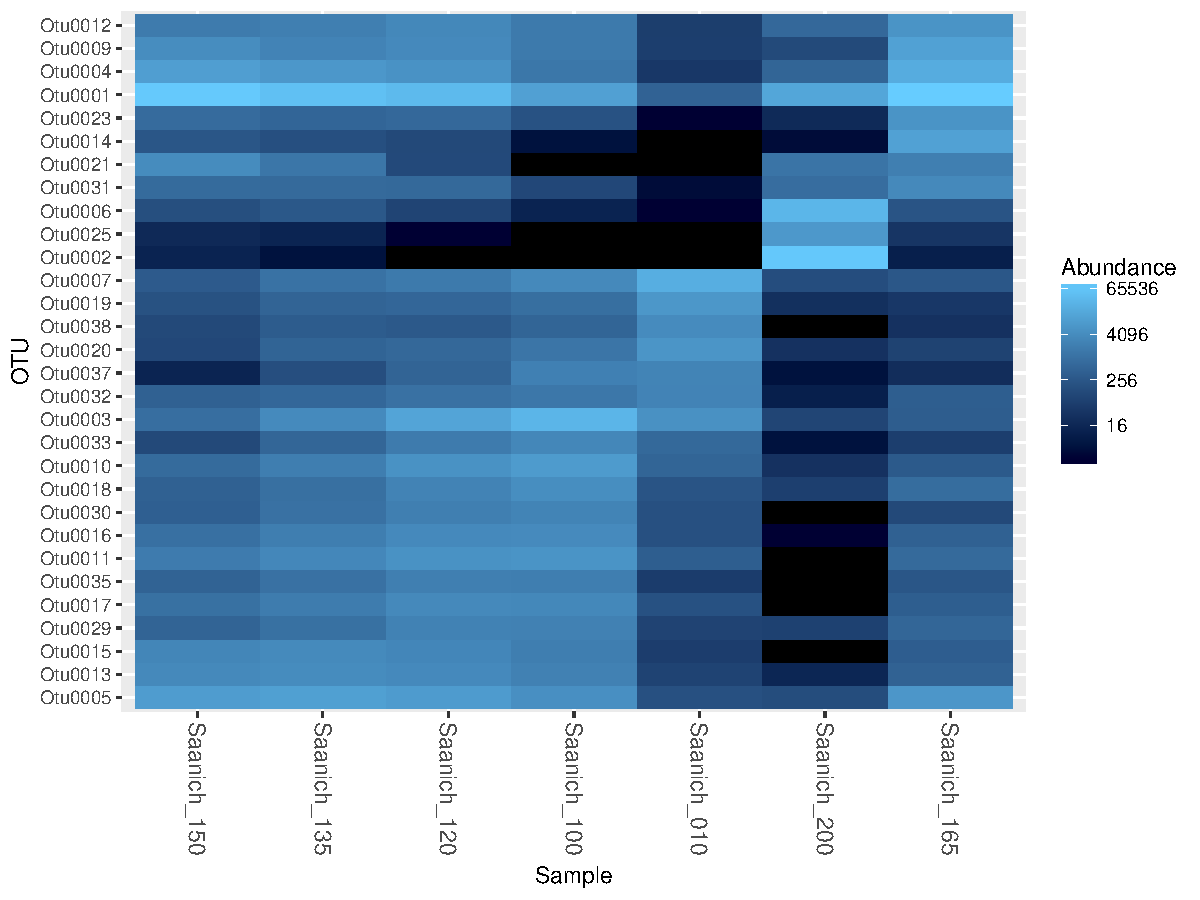
\includegraphics{Figs/unnamed-chunk-9-1.pdf}

To observe similarities between samples and OTUs, we apply the
follwoing:

\begin{Shaded}
\begin{Highlighting}[]
\KeywordTok{heatmap}\NormalTok{(}\KeywordTok{otu_table}\NormalTok{(prunedTaxa))}
\end{Highlighting}
\end{Shaded}

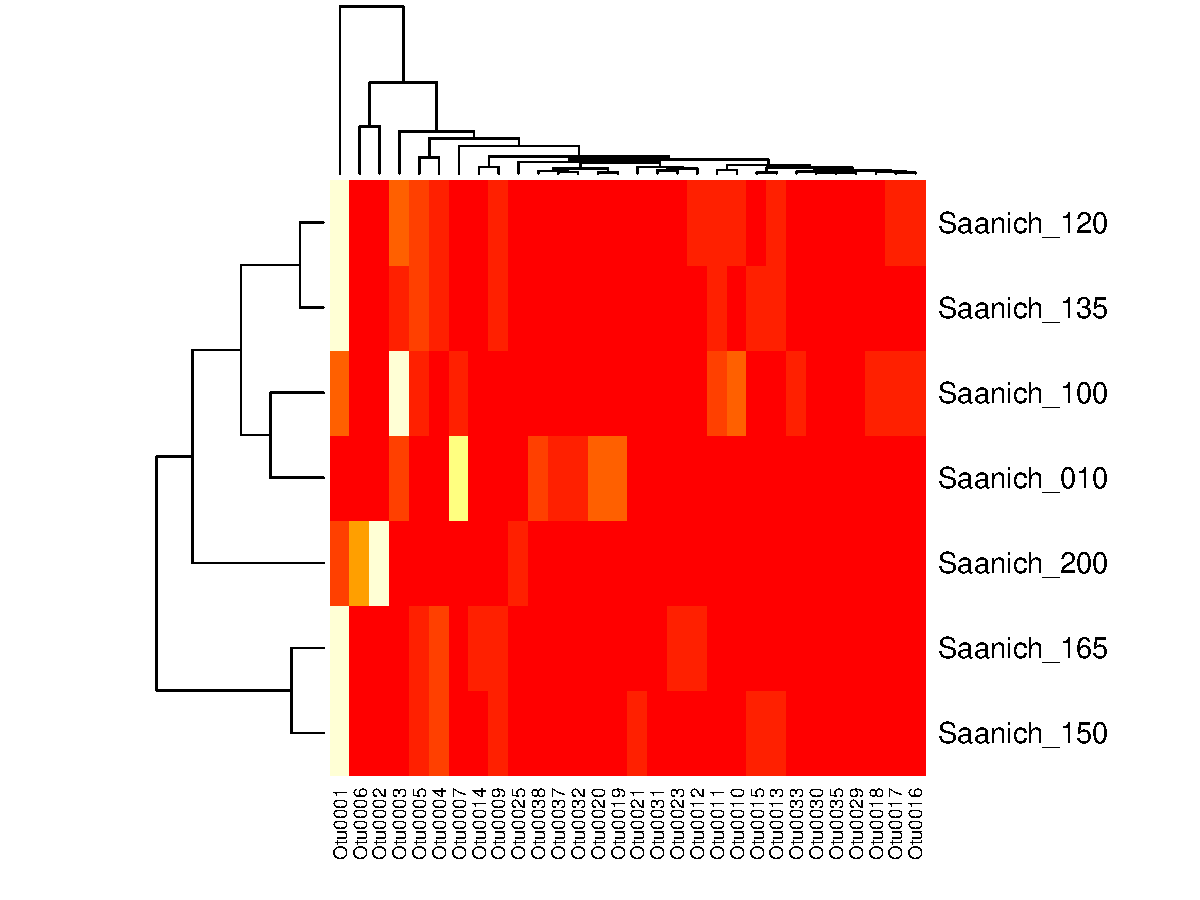
\includegraphics{Figs/unnamed-chunk-10-1.pdf}

The following function will assist us to understand the unique Phylum
rank:

\begin{Shaded}
\begin{Highlighting}[]
\KeywordTok{get_taxa_unique}\NormalTok{(}\DataTypeTok{physeq =}\NormalTok{ workingTaxa, }\DataTypeTok{taxonomic.rank =} \StringTok{"Phylum"}\NormalTok{)}
\end{Highlighting}
\end{Shaded}

\begin{verbatim}
## [1] "Proteobacteria"                "Bacteroidetes"                
## [3] "Thaumarchaeota"                "Actinobacteria"               
## [5] "Marinimicrobia_(SAR406_clade)" "Planctomycetes"               
## [7] "Gemmatimonadetes"              "Verrucomicrobia"              
## [9] "Chloroflexi"
\end{verbatim}

We choose the \emph{Planctomycetes} phylum and we explore the
distribution of genera of this phylum.

\begin{Shaded}
\begin{Highlighting}[]
\NormalTok{subTaxa =}\StringTok{ }\KeywordTok{subset_taxa}\NormalTok{(workingTaxa, Phylum }\OperatorTok{==}\StringTok{ "Planctomycetes"}\NormalTok{)}
\KeywordTok{plot_bar}\NormalTok{(subTaxa, }\DataTypeTok{fill=}\StringTok{"Genus"}\NormalTok{)}
\end{Highlighting}
\end{Shaded}

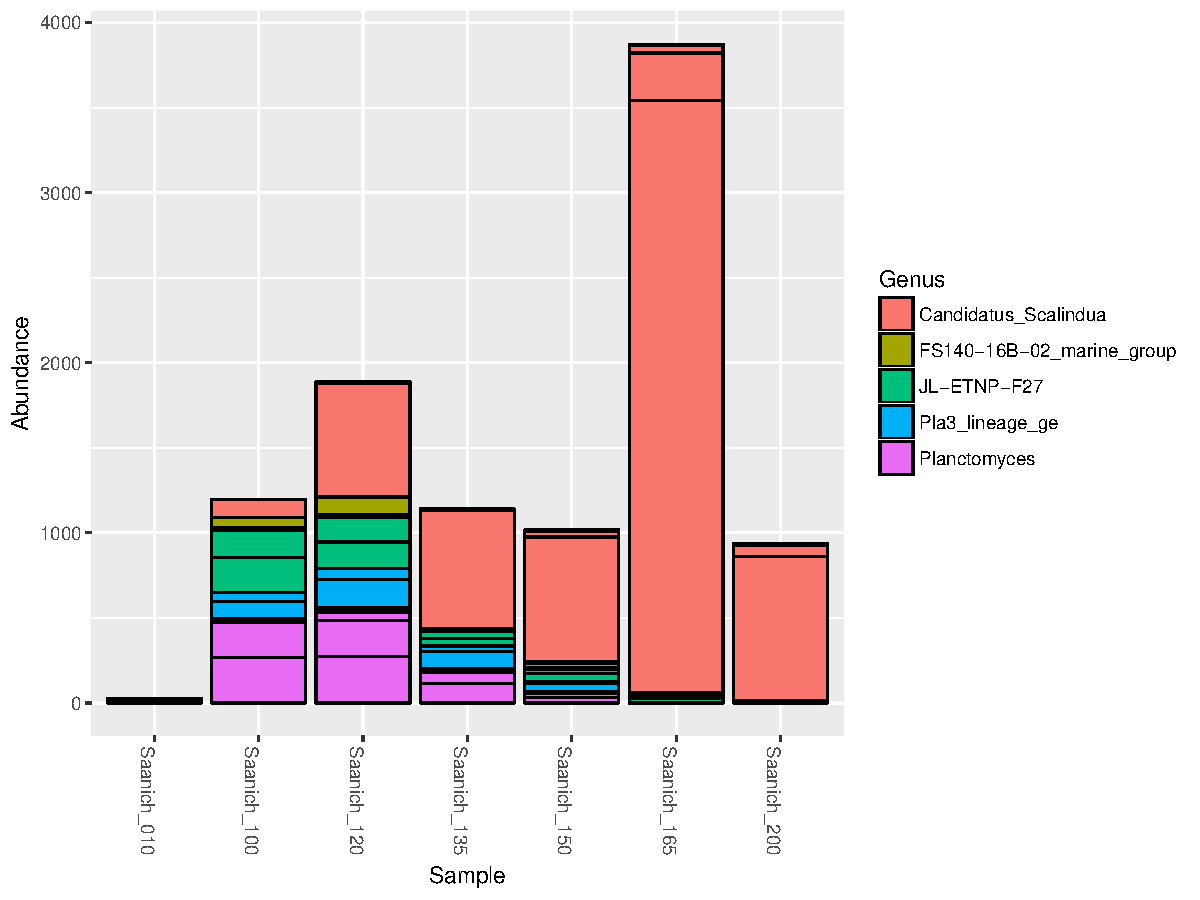
\includegraphics{Figs/unnamed-chunk-12-1.pdf}

We explore how the genus of this phulm varies across samples
(represnting depth of the ocean) based on genus abundances.

\begin{Shaded}
\begin{Highlighting}[]
\KeywordTok{plot_bar}\NormalTok{(subTaxa, }\StringTok{"Depth_m"}\NormalTok{, }\DataTypeTok{fill=}\StringTok{"Genus"}\NormalTok{, }\DataTypeTok{facet_grid=}\OperatorTok{~}\NormalTok{Family)}
\end{Highlighting}
\end{Shaded}

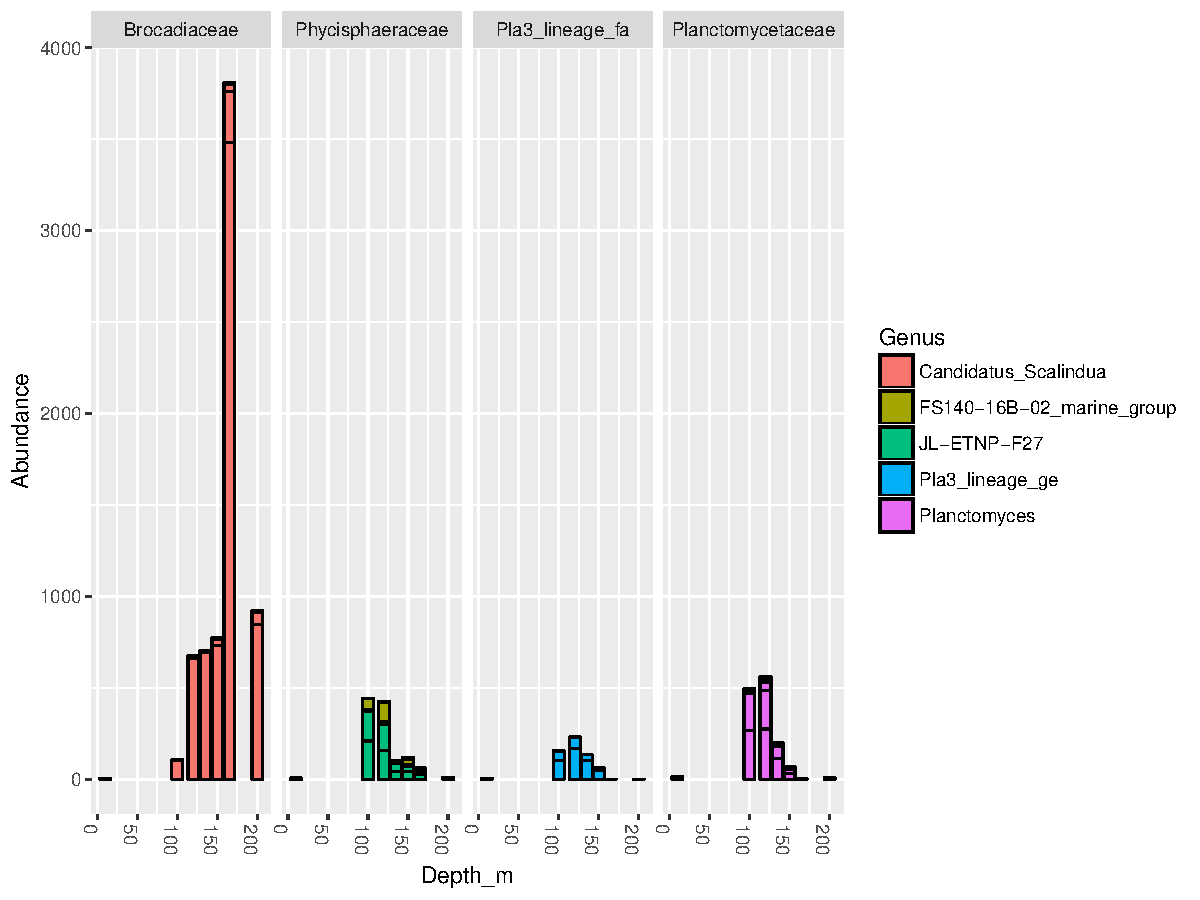
\includegraphics{Figs/unnamed-chunk-13-1.pdf}

The genus was chosen to be \emph{Planctomyces} and we identify the
following OTUs.

\begin{Shaded}
\begin{Highlighting}[]
\NormalTok{subGenTaxa =}\StringTok{ }\KeywordTok{subset_taxa}\NormalTok{(workingTaxa, Genus }\OperatorTok{==}\StringTok{ "Planctomyces"}\NormalTok{)}
\KeywordTok{colnames}\NormalTok{(}\KeywordTok{otu_table}\NormalTok{(subGenTaxa))}
\end{Highlighting}
\end{Shaded}

\begin{verbatim}
## [1] "Otu0125" "Otu0144" "Otu0401" "Otu0592" "Otu1038" "Otu1262"
\end{verbatim}

Estimate diversity of \emph{Planctomyces} across depth and oxygen
concentration.

\begin{Shaded}
\begin{Highlighting}[]
\KeywordTok{theme_set}\NormalTok{(}\KeywordTok{theme_bw}\NormalTok{())}
\NormalTok{pal =}\StringTok{ "Set1"}
\NormalTok{scale_colour_discrete <-}\StringTok{  }\ControlFlowTok{function}\NormalTok{(}\DataTypeTok{palname=}\NormalTok{pal, ...)\{}
  \KeywordTok{scale_colour_brewer}\NormalTok{(}\DataTypeTok{palette=}\NormalTok{palname, ...)}
\NormalTok{\}}
\NormalTok{scale_fill_discrete <-}\StringTok{  }\ControlFlowTok{function}\NormalTok{(}\DataTypeTok{palname=}\NormalTok{pal, ...)\{}
  \KeywordTok{scale_fill_brewer}\NormalTok{(}\DataTypeTok{palette=}\NormalTok{palname, ...)}
\NormalTok{\}}

\KeywordTok{plot_richness}\NormalTok{(workingTaxa, }\DataTypeTok{x=}\StringTok{"Depth_m"}\NormalTok{, }\DataTypeTok{color=}\StringTok{"Depth_m"}\NormalTok{, }\DataTypeTok{measures =} \KeywordTok{c}\NormalTok{(}\StringTok{"Chao1"}\NormalTok{, }\StringTok{"Shannon"}\NormalTok{, }\StringTok{"Simpson"}\NormalTok{)) }\OperatorTok{+}\StringTok{ }\KeywordTok{geom_point}\NormalTok{(}\DataTypeTok{size=}\DecValTok{5}\NormalTok{, }\DataTypeTok{alpha=}\FloatTok{0.7}\NormalTok{)}\OperatorTok{+}\StringTok{ }\KeywordTok{geom_line}\NormalTok{()}
\end{Highlighting}
\end{Shaded}

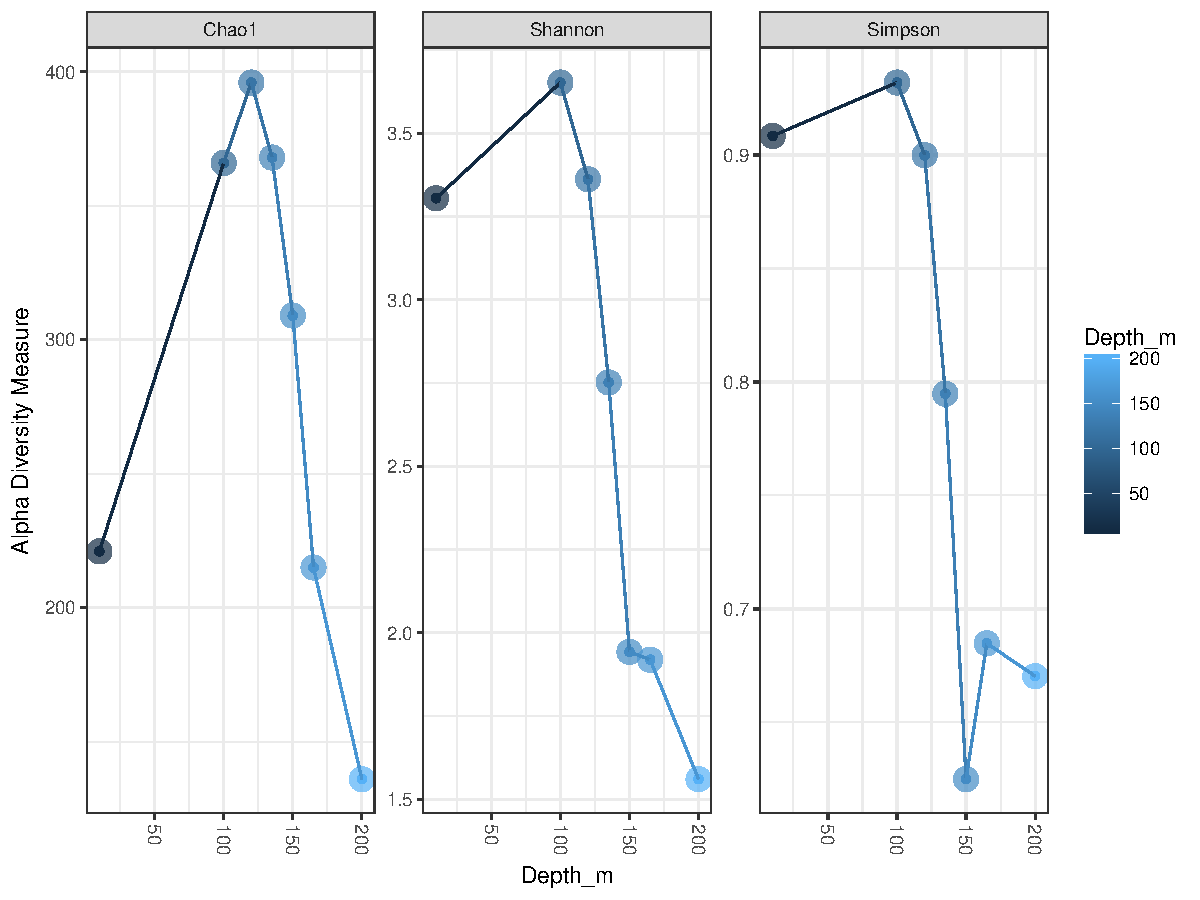
\includegraphics{Figs/unnamed-chunk-15-1.pdf}

\begin{Shaded}
\begin{Highlighting}[]
\KeywordTok{plot_richness}\NormalTok{(workingTaxa, }\DataTypeTok{x=}\StringTok{"O2_uM"}\NormalTok{, }\DataTypeTok{color=}\StringTok{"O2_uM"}\NormalTok{, }\DataTypeTok{measures =} \KeywordTok{c}\NormalTok{(}\StringTok{"Chao1"}\NormalTok{, }\StringTok{"Shannon"}\NormalTok{, }\StringTok{"Simpson"}\NormalTok{)) }\OperatorTok{+}\StringTok{ }\KeywordTok{geom_point}\NormalTok{(}\DataTypeTok{size=}\DecValTok{5}\NormalTok{, }\DataTypeTok{alpha=}\FloatTok{0.7}\NormalTok{) }\OperatorTok{+}\StringTok{ }\KeywordTok{geom_line}\NormalTok{()}
\end{Highlighting}
\end{Shaded}

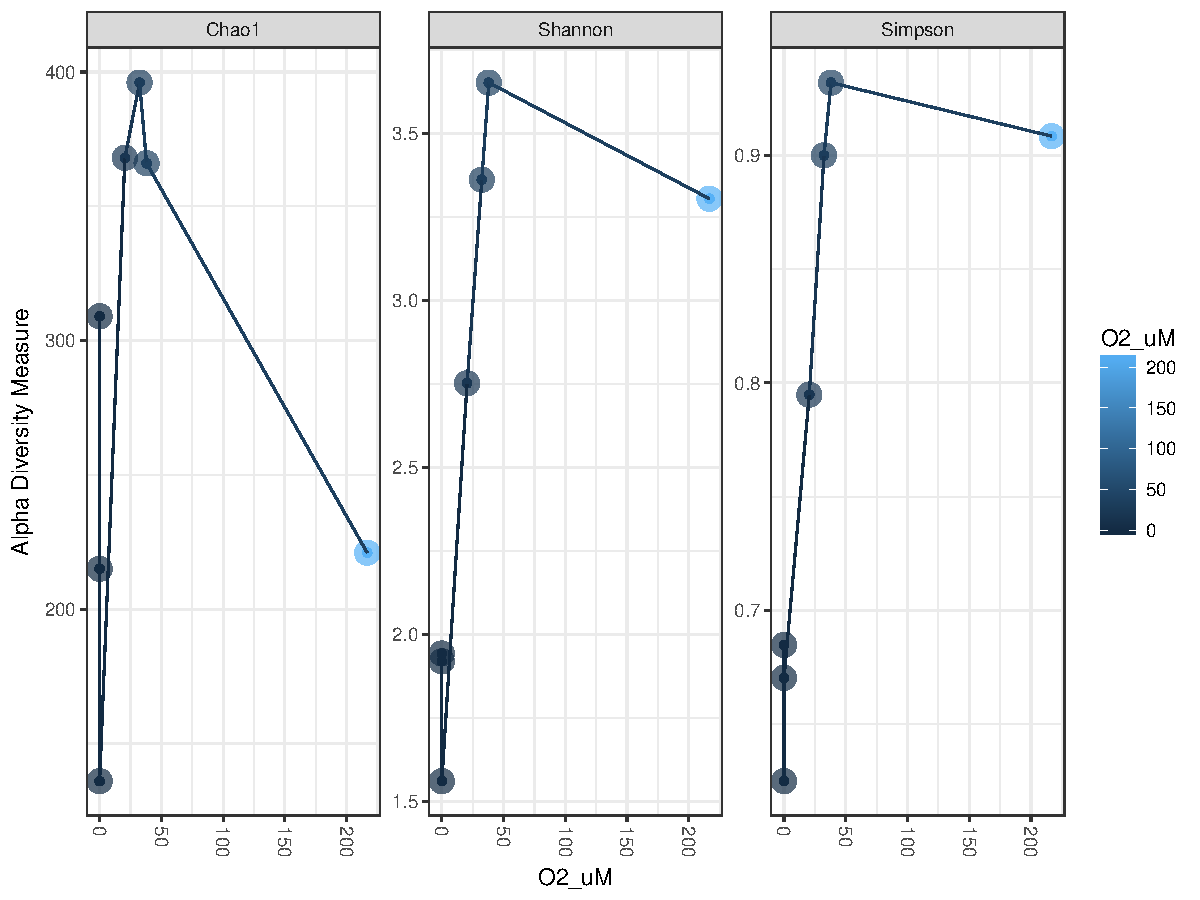
\includegraphics{Figs/unnamed-chunk-15-2.pdf}

\section{Results}\label{results}

\subsection{\texorpdfstring{Analysis of microbial community structure
along with depth and oxygen concentration
\label{sec:community}}{Analysis of microbial community structure along with depth and oxygen concentration }}\label{analysis-of-microbial-community-structure-along-with-depth-and-oxygen-concentration}

\subsection{\texorpdfstring{Analysis of abundance information of
{[}OTU****{]} along with depth and/or oxygen concentration
\label{sec:OTUabundance}}{Analysis of abundance information of {[}OTU****{]} along with depth and/or oxygen concentration }}\label{analysis-of-abundance-information-of-otu-along-with-depth-andor-oxygen-concentration}

\subsection{\texorpdfstring{Estimate richness (number of OTUs/ASVs) for
{[}OTU****{]}
\label{sec:richness}}{Estimate richness (number of OTUs/ASVs) for {[}OTU****{]} }}\label{estimate-richness-number-of-otusasvs-for-otu}

\subsection{\texorpdfstring{Interpretation of abundance information of
OTUs/ASVs of {[}OTU****{]} along with depth and/or oxygen concentration
\label{sec:ASVabundances}}{Interpretation of abundance information of OTUs/ASVs of {[}OTU****{]} along with depth and/or oxygen concentration }}\label{interpretation-of-abundance-information-of-otusasvs-of-otu-along-with-depth-andor-oxygen-concentration}

\section{Discussion}\label{discussion}

(Hawley et al. 2017; Torres-Beltrán et al. 2017)

\begin{center}\rule{0.5\linewidth}{\linethickness}\end{center}

\section*{References}\label{references}
\addcontentsline{toc}{section}{References}

\hypertarget{refs}{}
\hypertarget{ref-Hawley2017:compendium}{}
Hawley, Alyse K, Mónica Torres-Beltrán, Elena Zaikova, David A Walsh,
Andreas Mueller, Melanie Scofield, Sam Kheirandish, et al. 2017. ``A
Compendium of Multi-Omic Sequence Information from the Saanich Inlet
Water Column.'' \emph{Scientific Data} 4. Nature Publishing Group:
170160.

\hypertarget{ref-Torres2017:compendium}{}
Torres-Beltrán, Mónica, Alyse K Hawley, David Capelle, Elena Zaikova,
David A Walsh, Andreas Mueller, Melanie Scofield, et al. 2017. ``A
Compendium of Geochemical Information from the Saanich Inlet Water
Column.'' \emph{Scientific Data} 4. Nature Publishing Group: 170159.


\end{document}
